\documentclass{standalone}
\usepackage{tikz}
\usetikzlibrary{patterns, positioning}


\begin{document}
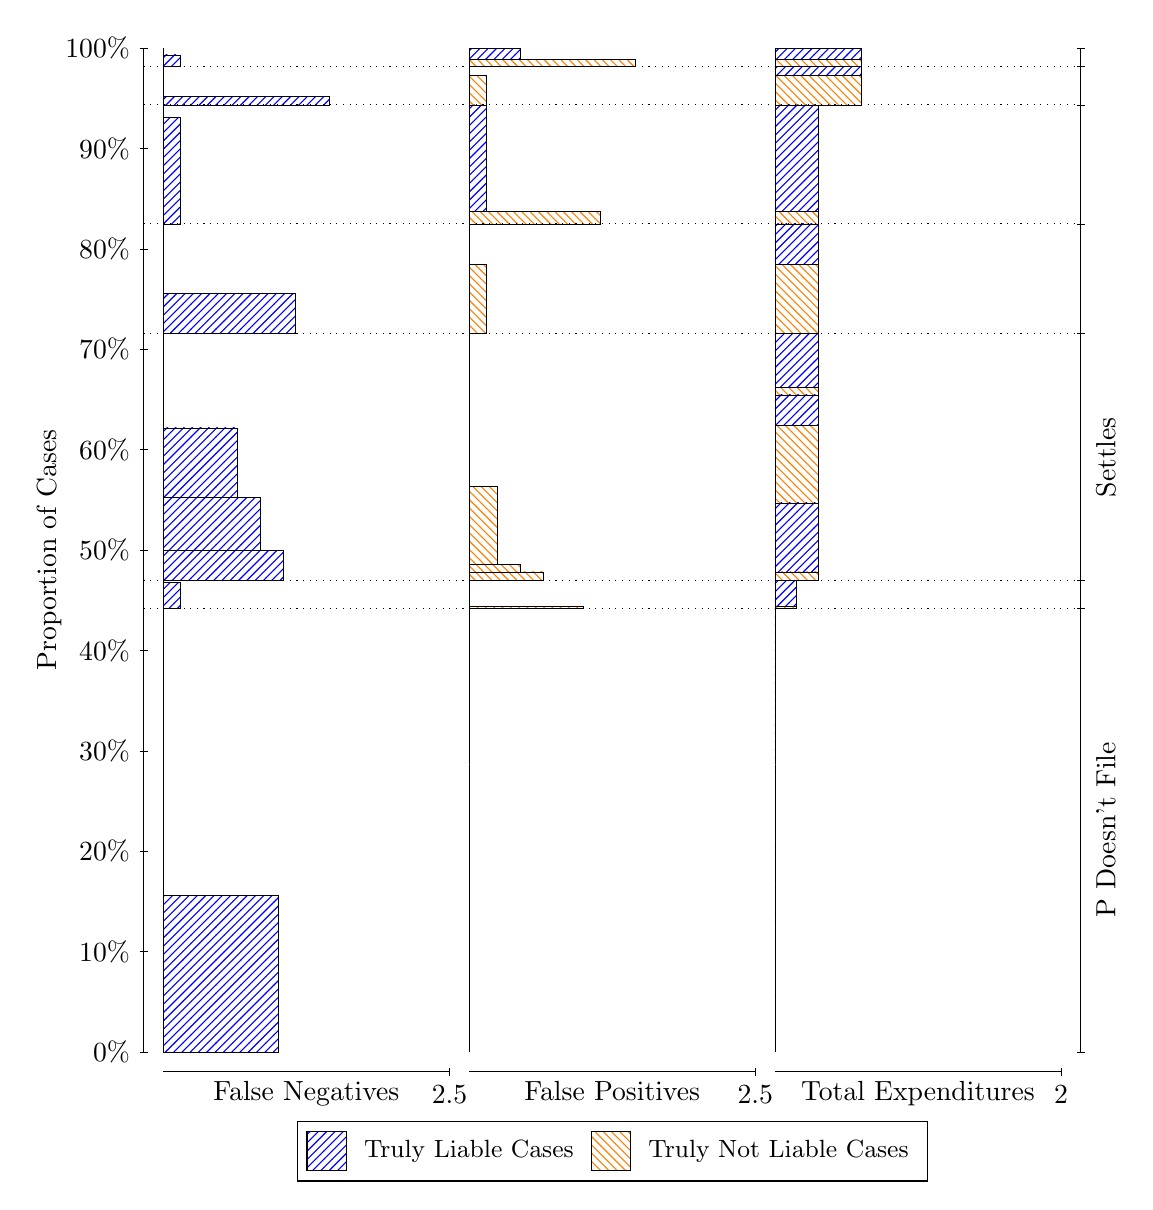
\begin{tikzpicture}
\draw[black, very thin] (1.5,1.75) -- (1.5,14.5);
\node[rotate=90, text=black, anchor=center] at (0.3, 8.125) {Proportion of Cases};
\draw[black, very thin] (1.45,1.75) -- (1.55,1.75);
\node[text=black, anchor=east] at (1.45, 1.75) {0\%};
\draw[black, very thin] (1.45,3.025) -- (1.55,3.025);
\node[text=black, anchor=east] at (1.45, 3.025) {10\%};
\draw[black, very thin] (1.45,4.3) -- (1.55,4.3);
\node[text=black, anchor=east] at (1.45, 4.3) {20\%};
\draw[black, very thin] (1.45,5.575) -- (1.55,5.575);
\node[text=black, anchor=east] at (1.45, 5.575) {30\%};
\draw[black, very thin] (1.45,6.85) -- (1.55,6.85);
\node[text=black, anchor=east] at (1.45, 6.85) {40\%};
\draw[black, very thin] (1.45,8.125) -- (1.55,8.125);
\node[text=black, anchor=east] at (1.45, 8.125) {50\%};
\draw[black, very thin] (1.45,9.4) -- (1.55,9.4);
\node[text=black, anchor=east] at (1.45, 9.4) {60\%};
\draw[black, very thin] (1.45,10.675) -- (1.55,10.675);
\node[text=black, anchor=east] at (1.45, 10.675) {70\%};
\draw[black, very thin] (1.45,11.95) -- (1.55,11.95);
\node[text=black, anchor=east] at (1.45, 11.95) {80\%};
\draw[black, very thin] (1.45,13.225) -- (1.55,13.225);
\node[text=black, anchor=east] at (1.45, 13.225) {90\%};
\draw[black, very thin] (1.45,14.5) -- (1.55,14.5);
\node[text=black, anchor=east] at (1.45, 14.5) {100\%};

\draw[black, very thin] (13.4,1.75) -- (13.4,14.5);
\draw[black, very thin] (13.35,1.75) -- (13.45,1.75);
\node[anchor=west] at (13.35, 1.75) {};
\draw[black, very thin] (13.35,7.3861) -- (13.45,7.3861);
\node[anchor=west] at (13.35, 7.3861) {};
\draw[black, very thin] (13.35,7.7355) -- (13.45,7.7355);
\node[anchor=west] at (13.35, 7.7355) {};
\draw[black, very thin] (13.35,10.872) -- (13.45,10.872);
\node[anchor=west] at (13.35, 10.872) {};
\draw[black, very thin] (13.35,12.268) -- (13.45,12.268);
\node[anchor=west] at (13.35, 12.268) {};
\draw[black, very thin] (13.35,13.778) -- (13.45,13.778);
\node[anchor=west] at (13.35, 13.778) {};
\draw[black, very thin] (13.35,14.266) -- (13.45,14.266);
\node[anchor=west] at (13.35, 14.266) {};
\draw[black, very thin] (13.35,14.5) -- (13.45,14.5);
\node[anchor=west] at (13.35, 14.5) {};

\draw[black, very thin, pattern color=blue, pattern=north east lines] (1.75,1.75) rectangle (3.2033,3.7351);
\draw[black, very thin, pattern color=orange, pattern=north west lines] (1.75,3.7351) rectangle (1.75,7.3861);
\draw[black, very thin, pattern color=blue, pattern=north east lines] (1.75,7.3861) rectangle (1.968,7.716);
\draw[black, very thin, pattern color=orange, pattern=north west lines] (1.75,7.716) rectangle (1.75,7.7355);
\draw[black, very thin, pattern color=blue, pattern=north east lines] (1.75,7.7355) rectangle (3.276,8.1196);
\draw[black, very thin, pattern color=blue, pattern=north east lines] (1.75,8.1196) rectangle (2.9853,8.7969);
\draw[black, very thin, pattern color=blue, pattern=north east lines] (1.75,8.7969) rectangle (2.6947,9.6747);
\draw[black, very thin, pattern color=orange, pattern=north west lines] (1.75,9.6747) rectangle (1.75,10.872);
\draw[black, very thin, pattern color=blue, pattern=north east lines] (1.75,10.872) rectangle (3.4213,11.387);
\draw[black, very thin, pattern color=orange, pattern=north west lines] (1.75,11.387) rectangle (1.75,12.268);
\draw[black, very thin, pattern color=blue, pattern=north east lines] (1.75,12.268) rectangle (1.968,13.616);
\draw[black, very thin, pattern color=orange, pattern=north west lines] (1.75,13.616) rectangle (1.75,13.778);
\draw[black, very thin, pattern color=blue, pattern=north east lines] (1.75,13.778) rectangle (3.8573,13.89);
\draw[black, very thin, pattern color=orange, pattern=north west lines] (1.75,13.89) rectangle (1.75,14.266);
\draw[black, very thin, pattern color=blue, pattern=north east lines] (1.75,14.266) rectangle (1.968,14.412);
\draw[black, very thin, pattern color=orange, pattern=north west lines] (1.75,14.412) rectangle (1.75,14.5);
\draw[black, very thin, pattern color=orange, pattern=north west lines] (5.6333,1.75) rectangle (5.6333,5.401);
\draw[black, very thin, pattern color=blue, pattern=north east lines] (5.6333,5.401) rectangle (5.6333,7.3861);
\draw[black, very thin, pattern color=orange, pattern=north west lines] (5.6333,7.3861) rectangle (7.0867,7.4056);
\draw[black, very thin, pattern color=blue, pattern=north east lines] (5.6333,7.4056) rectangle (5.6333,7.7355);
\draw[black, very thin, pattern color=orange, pattern=north west lines] (5.6333,7.7355) rectangle (6.578,7.8457);
\draw[black, very thin, pattern color=orange, pattern=north west lines] (5.6333,7.8457) rectangle (6.2873,7.9451);
\draw[black, very thin, pattern color=orange, pattern=north west lines] (5.6333,7.9451) rectangle (5.9967,8.933);
\draw[black, very thin, pattern color=blue, pattern=north east lines] (5.6333,8.933) rectangle (5.6333,10.872);
\draw[black, very thin, pattern color=orange, pattern=north west lines] (5.6333,10.872) rectangle (5.8513,11.753);
\draw[black, very thin, pattern color=blue, pattern=north east lines] (5.6333,11.753) rectangle (5.6333,12.268);
\draw[black, very thin, pattern color=orange, pattern=north west lines] (5.6333,12.268) rectangle (7.3047,12.429);
\draw[black, very thin, pattern color=blue, pattern=north east lines] (5.6333,12.429) rectangle (5.8513,13.778);
\draw[black, very thin, pattern color=orange, pattern=north west lines] (5.6333,13.778) rectangle (5.8513,14.154);
\draw[black, very thin, pattern color=blue, pattern=north east lines] (5.6333,14.154) rectangle (5.6333,14.266);
\draw[black, very thin, pattern color=orange, pattern=north west lines] (5.6333,14.266) rectangle (7.7407,14.354);
\draw[black, very thin, pattern color=blue, pattern=north east lines] (5.6333,14.354) rectangle (6.2873,14.5);
\draw[black, very thin, pattern color=orange, pattern=north west lines] (9.5167,1.75) rectangle (9.5167,5.401);
\draw[black, very thin, pattern color=blue, pattern=north east lines] (9.5167,5.401) rectangle (9.5167,7.3861);
\draw[black, very thin, pattern color=orange, pattern=north west lines] (9.5167,7.3861) rectangle (9.7892,7.4056);
\draw[black, very thin, pattern color=blue, pattern=north east lines] (9.5167,7.4056) rectangle (9.7892,7.7355);
\draw[black, very thin, pattern color=orange, pattern=north west lines] (9.5167,7.7355) rectangle (10.062,7.8457);
\draw[black, very thin, pattern color=blue, pattern=north east lines] (9.5167,7.8457) rectangle (10.062,8.7235);
\draw[black, very thin, pattern color=orange, pattern=north west lines] (9.5167,8.7235) rectangle (10.062,9.7114);
\draw[black, very thin, pattern color=blue, pattern=north east lines] (9.5167,9.7114) rectangle (10.062,10.095);
\draw[black, very thin, pattern color=orange, pattern=north west lines] (9.5167,10.095) rectangle (10.062,10.195);
\draw[black, very thin, pattern color=blue, pattern=north east lines] (9.5167,10.195) rectangle (10.062,10.872);
\draw[black, very thin, pattern color=orange, pattern=north west lines] (9.5167,10.872) rectangle (10.062,11.753);
\draw[black, very thin, pattern color=blue, pattern=north east lines] (9.5167,11.753) rectangle (10.062,12.268);
\draw[black, very thin, pattern color=orange, pattern=north west lines] (9.5167,12.268) rectangle (10.062,12.429);
\draw[black, very thin, pattern color=blue, pattern=north east lines] (9.5167,12.429) rectangle (10.062,13.778);
\draw[black, very thin, pattern color=orange, pattern=north west lines] (9.5167,13.778) rectangle (10.607,14.154);
\draw[black, very thin, pattern color=blue, pattern=north east lines] (9.5167,14.154) rectangle (10.607,14.266);
\draw[black, very thin, pattern color=orange, pattern=north west lines] (9.5167,14.266) rectangle (10.607,14.354);
\draw[black, very thin, pattern color=blue, pattern=north east lines] (9.5167,14.354) rectangle (10.607,14.5);
\draw[black, dotted] (1.5,7.3861) -- (13.4,7.3861);
\draw[black, dotted] (1.5,7.7355) -- (13.4,7.7355);
\draw[black, dotted] (1.5,10.872) -- (13.4,10.872);
\draw[black, dotted] (1.5,12.268) -- (13.4,12.268);
\draw[black, dotted] (1.5,13.778) -- (13.4,13.778);
\draw[black, dotted] (1.5,14.266) -- (13.4,14.266);
\draw[black, very thin] (1.75,1.5) -- (5.3833,1.5);
\node[text=black, anchor=north] at (3.5667, 1.5) {False Negatives};
\draw[black, very thin] (5.3833,1.45) -- (5.3833,1.55);
\node[text=black, anchor=north] at (5.3833, 1.45) {2.5};

\draw[black, very thin] (5.6333,1.5) -- (9.2667,1.5);
\node[text=black, anchor=north] at (7.45, 1.5) {False Positives};
\draw[black, very thin] (9.2667,1.45) -- (9.2667,1.55);
\node[text=black, anchor=north] at (9.2667, 1.45) {2.5};

\draw[black, very thin] (9.5167,1.5) -- (13.15,1.5);
\node[text=black, anchor=north] at (11.333, 1.5) {Total Expenditures};
\draw[black, very thin] (13.15,1.45) -- (13.15,1.55);
\node[text=black, anchor=north] at (13.15, 1.45) {2};

\node[text=black, centered, rotate=90] at (13.72, 4.5681) {P Doesn't File};

\node[text=black, centered, rotate=90] at (13.72, 9.3038) {Settles};





\draw (7.449999999999999,1.5) node[draw=none] (baseCoordinate) {};
\begin{scope}[align=center]
        \matrix[scale=0.5, draw=black, below=0.5cm of baseCoordinate, nodes={draw}, column sep=0.1cm]{
            \node[rectangle, draw, minimum width=0.5cm, minimum height=0.5cm, pattern color=blue, pattern=north east lines] {}; &
            \node[draw=none, font=\small, text=black] (B) {Truly Liable Cases}; &
            \node[rectangle, draw, minimum width=0.5cm, minimum height=0.5cm, pattern color=orange, pattern=north west lines] {}; &
            \node[draw=none, font=\small, text=black] (B) {Truly Not Liable Cases}; \\
            };
\end{scope}

\end{tikzpicture}
\end{document}